\documentclass[../main.tex]{subfiles}
\begin{document}
The chapter report the development process for the software dashboard, starting from explaining the requirements behind the needs of a software dashboard and how this helps developer in the process of generating software for motor \gls{ECUM}s. The chapter report the path towards the construction of the dashboard following the flow that the data has inside the pipeline that brings always updating data to the dashboard itself. The first part discuss the software structure at \gls{BMW} and the data related to it, then the code that generated this data is reported, keeping an eye on the data side of this. Concluding the chapter report the pipeline implementations and the details related to the dashboard itself.
\section{Dashboard objective definition}
As already introduced in the Thesis abstract the development of \gls{ECU} software is complex process. As each complex process composed by multiple step there is always the requirement of tracking results, quality and completeness of each step. In order to do that a high load of data is generated during each step in order to have a feedback on the status of execution.\\
In the development of \gls{ECU} software most of the steps to create software are divided on multiple departments and then additionally divided between the single member of a team. Each of the person responsible for a single task keep track of the data of that single task. Most of the time only single person know where the data for the single task lay and also how to read those data. This can create problem especially when people outside the task require information for it. They always need to refer to the person in charge. A centralized view on the process is missing, as also a centralize storing repository for the data. \\
The idea to create a database to store data in a readable form and the to create graphical visualization, namely dashboard of the data, is the idea that want to full fill the previous raised problem.\\
Via a dashboard with updated data different developers in different teams can simultaneously surf thought the data and get real time information on the status of the process, thus increasing the feedback on every task and therefor the output result.
\subsection{Data pipeline concept}
The concept of having data flowing from the source that generates the data all the way to the dashboard can be summarized under the name pipeline. This gives an idea of the basic concept that the flow of data need to have. The data need to be always updated, the flow need to be controlled by some mechanism that take the updating data and push it to the different steps of the pipe all the way to the dashboard itself. Three main steps can be identified in the pipeline:

\tikzstyle{block} = [draw, rectangle, text width=3.5cm, text centered, minimum height=1.2cm, node distance=6cm]
\begin{figure}[h]
  \centering
\begin{tikzpicture}[scale=0.85,transform shape]
    \node [block, name=text1] {Data Source};
    \node [block, right of=text1] (text2) {Data Storage};
    \node [block, right of=text2] (text3) {Data Visualization};

    \draw [->] (text1) -- (text2);
    \draw [->] (text2) -- node {} (text3);

\end{tikzpicture}
  \caption{General pipeline structure}
  \label{pipelinestructure}
\end{figure}

\begin{itemize}
    \item Data source, in this case the data source is the EA-build software. As reported in Section \ref{sec:EA-buildsection} the software is responsible for the compilation of the code and therefor for the generation of the data. 
    \item Data storage, the data generate in the first process is stored in a relational database, namely EA-dashboard. This database is the middleman between the data source and the dashboard. The database receives information from the data source, stores the information under the form of tables and deliver data to the dashboard.
    \item Data visualization, the data stored in the database gets queried and reorganized. Visualization are created in a interactive manner in a dashboard available for the whole team.
\end{itemize}
\begin{figure}[h]
    \centering
    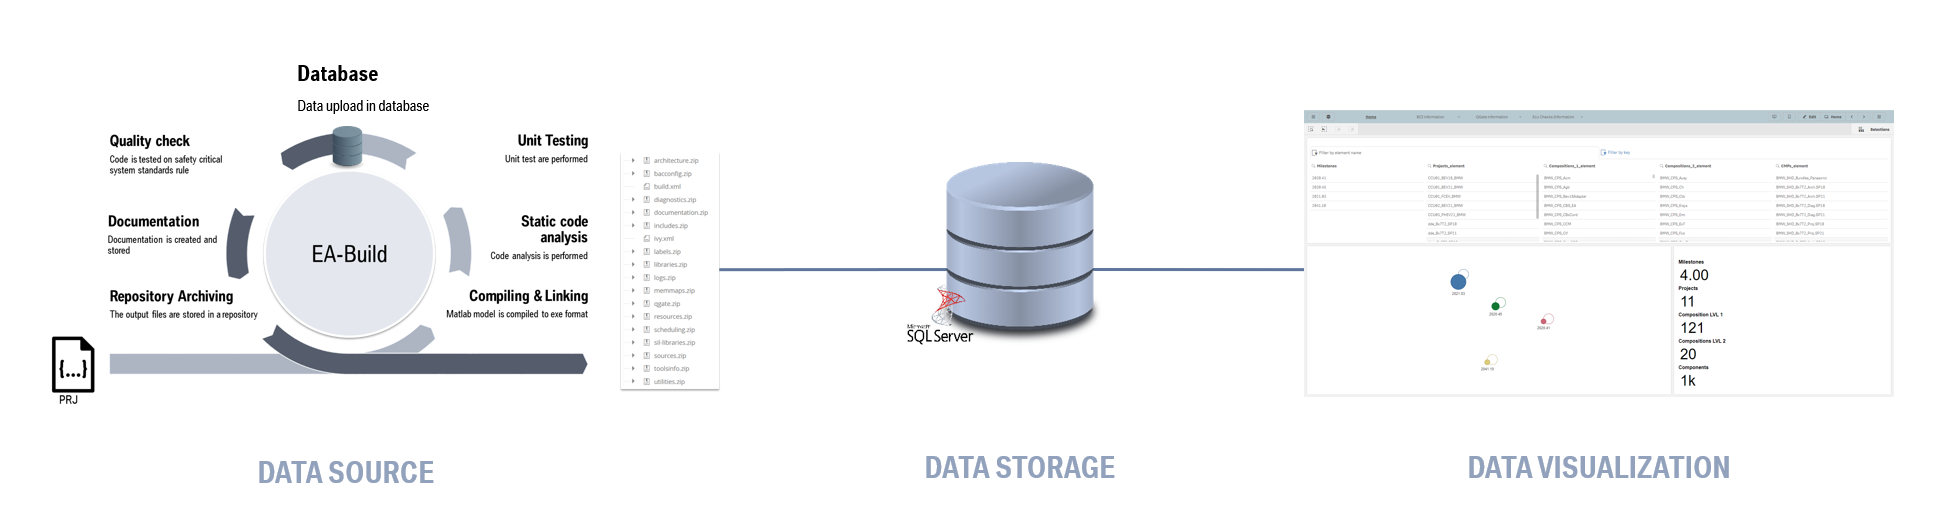
\includegraphics[width=\linewidth]{images_folder/pipeline_1.png}
    \caption{Pipeline structure}
    \label{fig:pipeline1}
\end{figure}
\section{Data Source}\label{sec:datasource}
The first part of the chapter introduce how the data is generated and what is the data related to software structure. Therefore during the section the software structure for \gls{ECU} is given and the data with an example of some batch data already integrated in the pipeline.
\subsection{Software structure for ECU}
In order to access and structure data there is the need of having a backbone structure, at which all the data can be related and can also be used to easily surf thought the data to search for relevant information. In this regard the software structure for \gls{ECU}s comes really in hand.\\ 
Software for \gls{ECU} is not developed as a single package. Software in packages for motor functional areas, each package namely compositions. A composition can refer to the full ignition system control. Under this composition other can be found all the way to the single software components that control the flow of fuel.\\
In the structure the sum of different composition define a project. A project refer to a different engine. One level up from composition we find the milestones, those refer to the baseline at which the software is consider, as explained in the chapter over Software Management Configuration. In general a Milestone follow the Scrum cycles, but there can be differences. \\
\begin{figure}
    \centering
    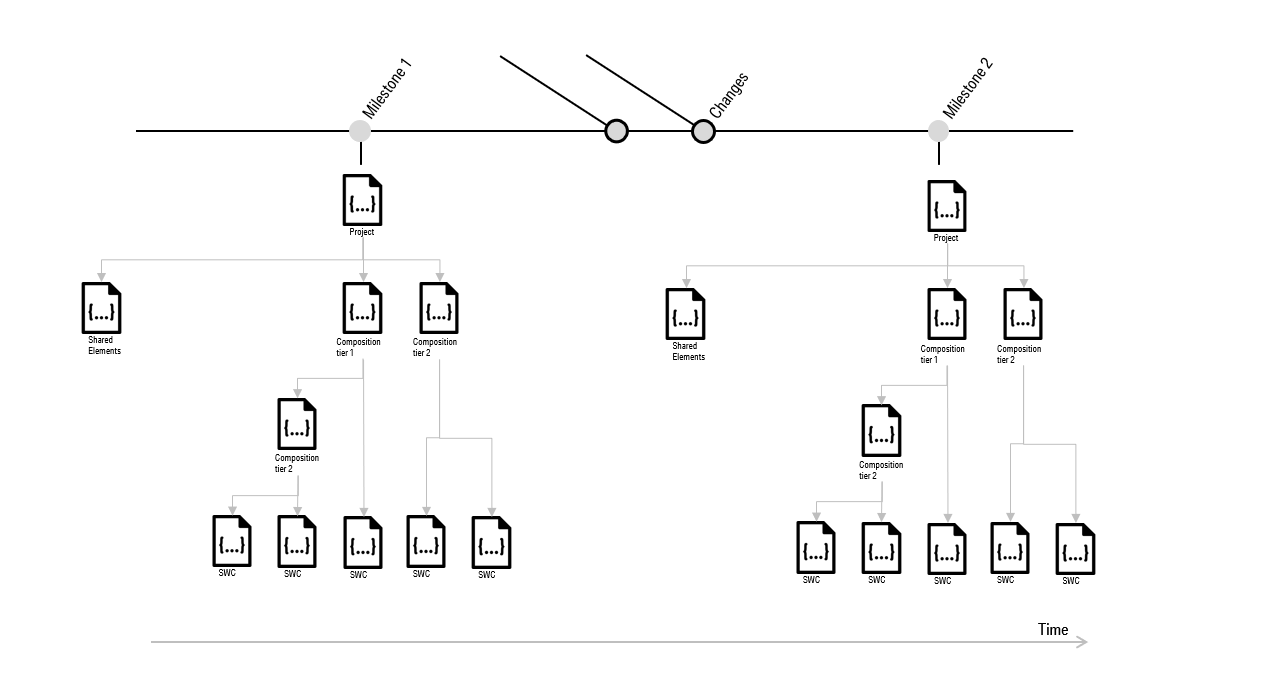
\includegraphics[width=\linewidth]{images_folder/softwarestrucutre.png}
    \caption{Software structure}
    \label{fig:SWsTR}
\end{figure}
\subsection{Automatic data generation}
the data generation process is the part of the project that is already present. the data is already there in the EA-build and gets generated every build run. Most of the time, as already mentioned the data gets stored under different formats, each of which is developer friendly, meaning that each developer know his own part of the data, and autonomously decides under which format to store the data under. 
In order to centralize the data the integration of the capabilities to store data in a database have been introduced in the build. The process for integration the automatic data generation to the database have been the following:
\begin{itemize}
    \item Creation of a database integration package, creation of a package to integrate database connectivity in the already present EA-build software.
    \item Standardization in the mechanism for database update, define a time efficient way to have always updating data and a constant timestamped storage. 
    \item Integration of data, workflow for the integration of new data inside the database.
\end{itemize}
\subsubsection{Creation of a database integration package}
whcih step are needed in tetrms - pythocn code, session creation, psw
The database package is the python package which inside the build process is responsible for storing the definition of table, following SQLAlchemy (Section \ref{sec:SQLACHMEYMSEC}).
The structure that allow to have a data going thought the software to the database is the following:
\begin{itemize}
    \item Each table has a class, based on \gls{ORM} layer creates a connection between the database table and the python native class. 
    \item A class responbile for storing connection parameter is present, in this class are stored information such as the ip address of the database, the port as well as the user for the server and database access. Different table uses different users related to different database schemas. 
    \item Each conncetion has a own sempathore on the flow stream, that is the so-called \texttt{Session}, that creates a holding zone for the created objects. 
        \lstset{language=Python}
        \lstset{frame=lines}
        \lstset{caption={Example of Session usage}}
        \lstset{label={lst:code_direct}}
        \lstset{basicstyle=\footnotesize}
        \begin{lstlisting}
            from sqlalchemy.orm import Session
            
            # create session and add objects
            with Session(someclass.engine) as session:
                session.add(some_object)
                session.add(some_other_object)
                session.commit()
        \end{lstlisting}
\end{itemize}
\subsubsection{Standardization of the database update mechanism}
Most of the data in the dashboard has an update periodicity of twenty minutes. This is related to the fact that update or changes in the software that trigger a rebuild, as reported in Section \ref{sec:CIsec}. This mean that the data to store exponentially. Therefor having a fast updating mechanism in the classic form, that checks what data is present and update only the data that changes is not feasible, or mostly not needed since in the dashboard the main focus is on a feedback directed to the current status of the software.
Based on those idea the update mechanism has been translated to a renew mechanism. With the term renew mean that the tables gets fully overwritten every times new data comes in. Thus deleting old data and updating as a bulk the new one.\\
It need to be underlined that the storage requirement highlighted at the beginning are still valid. Thus to full-fill this requirement, while keeping the data volume on the "production database" as low as possible a second database instance is created, namely "EA-Dashboard-storage". This database is updated from the "production" database once day, creating copies of all the tables and adding time stamping to the data, in order to keep track of the software status not only in a real time manner but also by having historic data on software versions. This database is not still connected to any dashboard or visualization. Therefor is as of today not possible to check the time evolution of the data. 
\begin{figure}
    \centering
    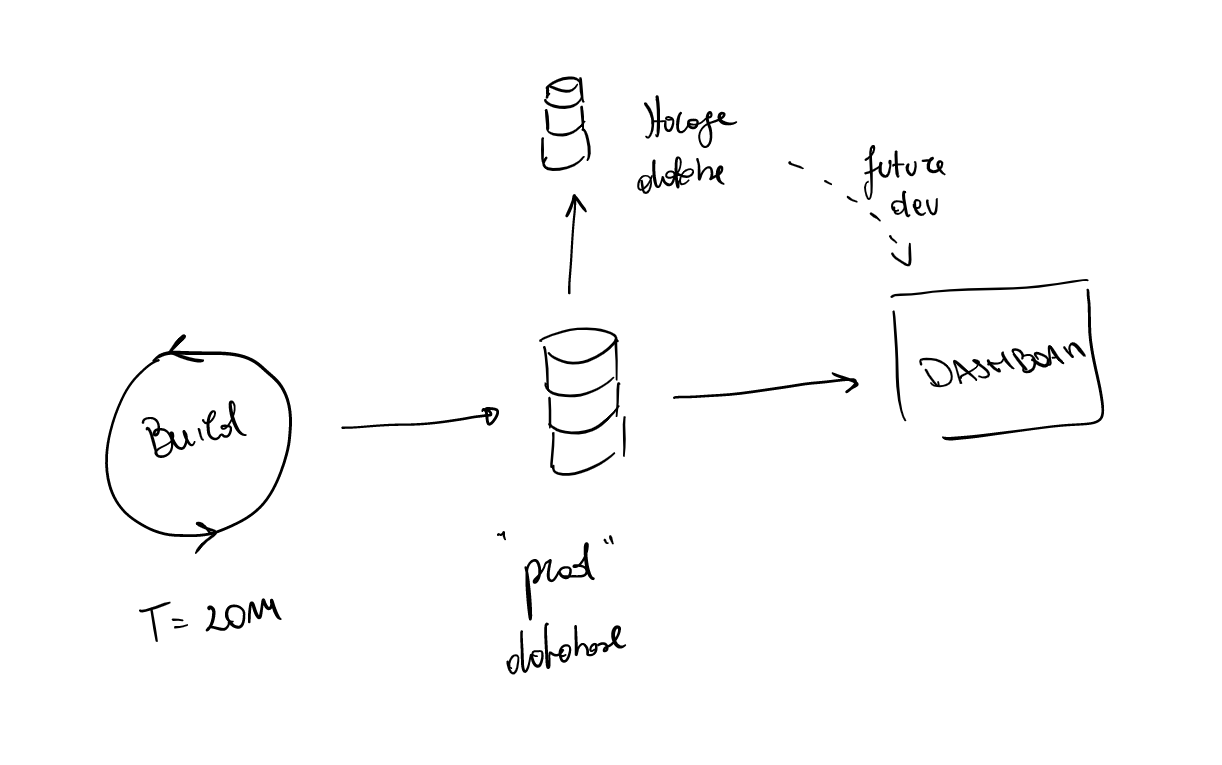
\includegraphics[width=\linewidth]{images_folder/dual_db.png}
    \caption{Double database structure}
    \label{fig:dds}
\end{figure}
\subsubsection{Integration of data}
In order to have new data inside the database and therefore flowing to the pipeline to be analyzed an showcased in a graphical manner in the dashboard some steps are required. Once the developer, together with the person in charge of the dashboard development decide that new data can be inserted in the process, thanks to the previously underline point the process is the following:
\begin{itemize}
    \item The developer highlight the data to the person in charge of integration, the main point that need to discussed is how the data gets connected to the data already present in the pipeline (choice of primary key)
    \item The integration person creates a class for the new data, that connect to a table object in the database. The class is then integrated in the code part that generate the data, so that once the data is generated this is also send to the database.
    \item The last step to full integration is adding a task, most of the time, based on Scons \ref{ssec:scon12} architecture, the right organization expect a task for each action, therefor the database integration is a new task, that is consequent to the data creation one, therefor the task need to be inserted in the application \texttt{.process} file, which defines which and how tasks run. 
\end{itemize}
\section{Data storage}
In the following section the database organization and structure is presented. This includes how the table are handled in the database and the mechanism behind structural organization
\subsection{Database table structure}
The requirements behind the first implementation in the production environment, coming from the product owner of the software in relation to the database integration were the following. Minimum changes in the production software allowed, this relates mainly to the data source (\ref{sec:datasource}) but greatly affect the complexity level allowed in the database organisation itself. Just to give an idea data can not be manipulated directly in the python code ,but need to be take as it is and then manipulated in the last step, data visualization. 
\begin{figure}[H]
    \centering
    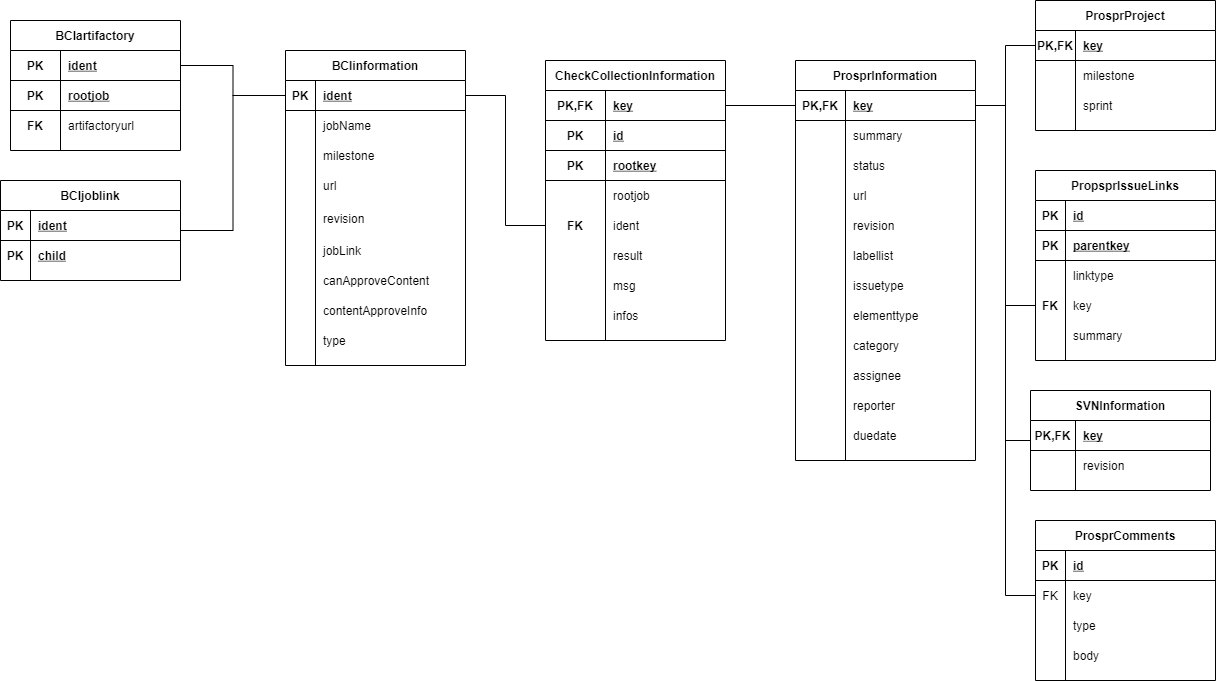
\includegraphics[width=\linewidth]{images_folder/EADBEntity.png}
    \caption{Database structure concept}
    \label{fig:dbsterconce}
\end{figure}
given this constraints the structure in the database is simplistic, the main flaw that required a second data organization via SQL queries is related to the fact that the data is taken as it is in code, so most of the time in an unstructured format. In Figure \ref{fig:dbsterconce} the first structure given in the database can be seen.
\begin{figure}[H]
    \centering
    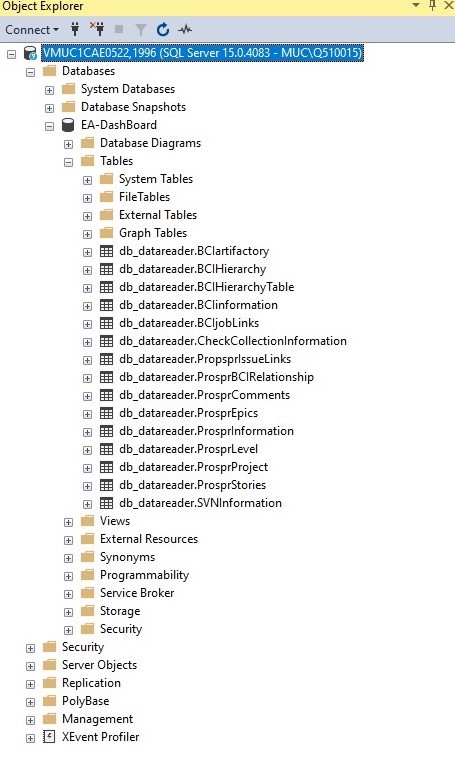
\includegraphics[width=0.5\linewidth]{images_folder/databasetable.jpg}
    \caption{Database tables}
    \label{fig:dbtables}
\end{figure} 

\section{Data Visualization}
In this section the data visualization tool is presented, as well as the concept used to create a visualization. 
\subsection{QlikSense}
QlikSense is a data analytic platform used to create interactive dashboards and reports. The tools allow connection with different data type, from excel sheets to database and via a SQL like language allow to query and manipulate data to create structured tables. From the structured table is then possible to create graphical visualisation of the data with interactive data search. The tool allow to develop interactive dashboard without the need of coding the graphic logic, but just the data structure behind the visualization.\\
The tool is structured in three main parts, that follow the data flow from raw data to the output dashboard and reports for customer or stakeholders:
\begin{itemize}
    \item Prepare, part in which the data is loaded and the table structure is created via a SQL flavored language. 
    \item Analyze, part in which the visualization is created, different visualization schemes and menu are presents. The graphic is mainly drag and drop but allow for a python like scripting to interface and insert formulas and conditions in the graphics.
    \item Narrate, part in which reports can be created form the dashboard. Reporting ability is crucial to have report arriving directly to the developer.  
\end{itemize}
\subsection{Double primary key layer}
Since QlikSense allow for a SQL like table structuring, based on table connected via key during the project it has been decided to manipulate the data in the QlikSense environment.\\
This allows to keep the structure in the database simple, thus avoiding having data manipulation in the Python, which is used in production to create \gls{ECU} deliverable. Having the lowest possible impact on the software, especially in the production environment was one of the first quest upon which the whole pipeline development was based.\\
Since data storage is not the first of the goal of the EA-build (Section \ref{sec:EA-buildsection}) keeping the part of the pipeline that connect the data generation and storage light as possible can be implemented. 
The data structuring is done in QlikSense via the SQL like code. The tables are loaded from the database and then modified. An example is reported in Figure \ref{fig:doublelayer}, where the software structure is imported in a parent in parent child manner. The hierarchical structure is then created via SQL queries in QlikSense.  
\begin{figure}[H]
    \centering
    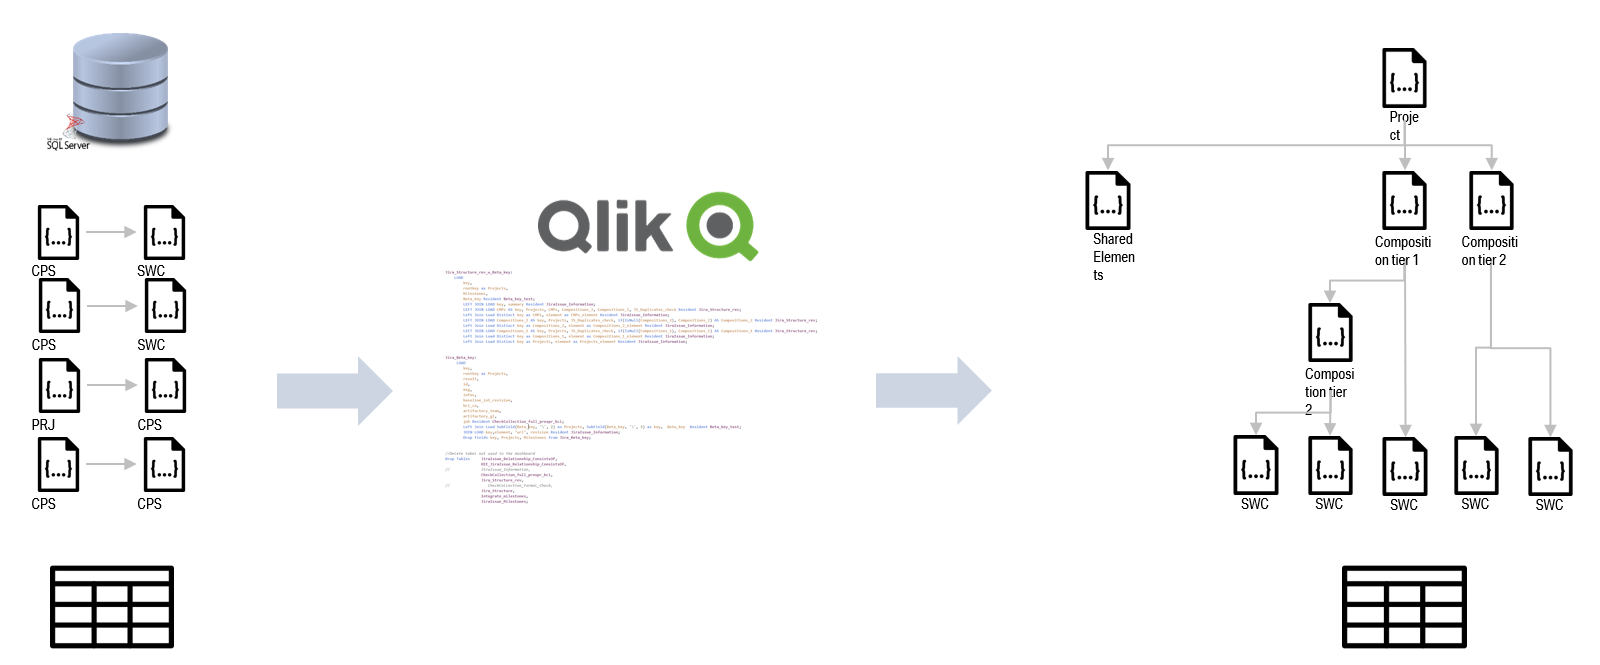
\includegraphics[width=\linewidth]{images_folder/doublalayer.png}
    \caption{Double layer primary key}
    \label{fig:doublelayer}
\end{figure} 
The concept of double layering for primary keys reports the idea that a primary key is defined both in the relational database environment. This primary key has the function of handling the update from the data generation, in terms that does not allow double data to be uploaded and define a initial data structure, not related to the visualization. The table in the database are uploaded as single instances in the QlikSense environment. Here a second primary key is defined, connecting the reorganized data. This primary key is the one in charge of connecting the data and allowing for for surfing thought the data in a interactive way. 
Using a double primary key layering allows, therefor for the following advantages:
\begin{itemize}
\item Have less changes in the production code for integrating the database connection and data generation.
\item During test and development phases having code defining the primary key connection in the QlikSense environment allow for a more flexibility, especially considering that in a database environment is more complex to redefine the table primary key. 
\end{itemize}
\subsection{EA Software dashboard}
\cleardoublepage
\end{document}